\chapter{Reference Implementation}
\label{chp:ReferenceImplementation}

The reference implementation of Epsilon provides execution engines for the languages and the orchestration workflow and end-user development tools that enable users to compose and execute Epsilon programs and workflows.

Java \cite{Java} has been selected as the language of choice for the implementation of Epsilon for a number of reasons; Java is a robust object-oriented language that can be executed in a wide range of software and hardware platforms, there are high-quality open-source development tools (such as the Eclipse JDT \cite{Eclipse}) for composing, debugging and executing Java programs, and finally the most robust and widely used modelling frameworks (EMF and MDR) that Epsilon needed to interface with have been also implemented using Java.

This chapter presents an overview of the reference implementation and highlights noteworthy aspects and key decisions made in it. The rest of the chapter is organized as follows. Section \ref{sec:Implementation.ExecutionEngines} provides an overview of the mechanisms that are used to parse and execute Epsilon programs. Section \ref{sec:Implementation.ModellingTechnologies} enumerates the modelling technologies that are supported by the reference implementation. Sections \ref{sec:Implementation.DevelopmentTools} and \ref{sec:Implementation.Workflow} provides an overview of the Eclipse-based development tools through which users can compose and execute Epsilon programs and workflows. Finally, Section \ref{sec:Implementation.Timeline} discusses the evolution and availability of the reference implementation in time, from its initial versions to the time of writing this report (May 2008).

\section{Execution Engines}
\label{sec:Implementation.ExecutionEngines}

The reference implementation provides an execution engine for each language of the platform. As displayed in Figure \ref{fig:InterpreterArchitecture}, each execution engine consists of four parts: lexer, parser, model builder and interpreter. The \emph{lexer} and \emph{parser} components are responsible for parsing textual programs into abstract syntax trees (ASTs) \cite{DragonBook}. Although the lexer and parser for a language can be hand-crafted, they are typically generated from a higher-level artefact that describes the \emph{grammar} of the language. In this reference implementation, the robust and widely-used ANTLR \cite{ANTLR} parser generator tool has been used for this purpose. Thus, for each language in the platform, an ANTLR grammar has been specified and from this, the respective lexers and parsers have been automatically generated. The main reason for selecting ANTLR among other tools with similar functionality was that ANTLR (in versions 2.x) supports grammar-level inheritance and this feature made it possible to realize the inheritance relationship that exists between task-specific languages and EOL without duplicating the EOL grammar in each of the task-specific languages grammars.

After parsing the textual program into an AST, the high-level logical constructs of the language (e.g. transformation-rules in ETL, operations in EOL etc.) are extracted from the AST into the \emph{logical model} from the \emph{model builder} component. By contrast, lower-level constructs such as statements and expressions are maintained in the form of ASTs. Finally, the \emph{interpreter} is responsible for executing the hybrid model.

\begin{figure}
	\centering
		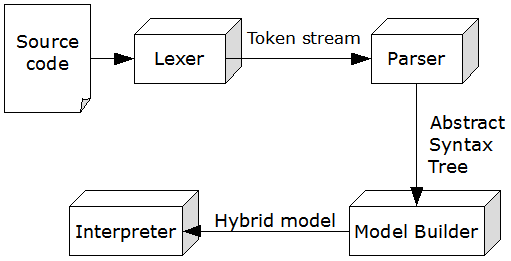
\includegraphics[width=0.7\textwidth]{images/InterpreterArchitecture.png}
	\caption{Overview of the Execution Engine of a typical Epsilon language}
	\label{fig:InterpreterArchitecture}
\end{figure}

The reason for this hybrid structure of the logical model (mixture of language-specific logical constructs and ASTs) and the use of interpreters instead of compilers is that the main concern in this exploratory reference implementation was modifiability and extensibility. Therefore, in prospect of the anticipated changes to the syntax and semantics of the languages that would - and did indeed - arise during the lifecycle of the project, it was decided that the most lightweight and flexible possible approach should be chosen.

However, the flexibility achieved with such a light-weight approach negatively affects attributes such as performance and usability. For example, a complete logical model for each language would arguably enhance performance and also enable static analysis which is necessary to implement usability enhancing features such as context aware code completion and detection of logical errors (e.g. accessing undefined properties). Since the syntax and semantics of the core and task-specific languages of the platform have been now stabilised, and thus they are not expected to change significantly, future versions of the implementation shall adopt the later approach to deliver improved performance and usability.

\section{Modelling Technologies}
\label{sec:Implementation.ModellingTechnologies}
The reference implementation contains EMC drivers (implementations of the \emph{IModel} interface discussed in Section \ref{sec:Design.EMC}) for the following modelling technologies. 

\begin{itemize}
	\item MOF 2.0, XMI 2.x using the Eclipse Modeling Framework (EMF)
	\item MOF 1.4, XMI 1.x using the Netbeans Metadata Repository (MDR)
	\item Plain XML
	\item Z, LaTeX (contributed by Wei Liu as part of an MSc thesis \cite{WeiLiu} that the author supervised)
\end{itemize}

The uniform access mechanism implemented by EMC enables model management programs expressed using languages in Epsilon to access and modify any number of models in these technologies in any combination (e.g. transform a MOF 1.4-based UML model to a Z model, compare a plain XML model with a MOF 2.0-based DSL model).

\section{Eclipse-based Development Tools}
\label{sec:Implementation.DevelopmentTools}
To be of practical use, each language in Epsilon is supported by a set of development tools built atop the Eclipse platform \cite{Eclipse}. This section provides a brief discussion on Eclipse and the Epsilon development tools implemented atop it. 

\subsection{The Eclipse Platform} 

Eclipse is an open-source software development framework supported by a large and active development and user community. As illustrated in Figure \ref{fig:EclipseArchitecture}, Eclipse adopts a modular architecture which consists of a small core and well-defined extension mechanisms that enable developers to contribute additional functionality in the form of \emph{plugins} (which can be grouped in the form of \emph{features} and \emph{products}).

\begin{figure}
	\centering
		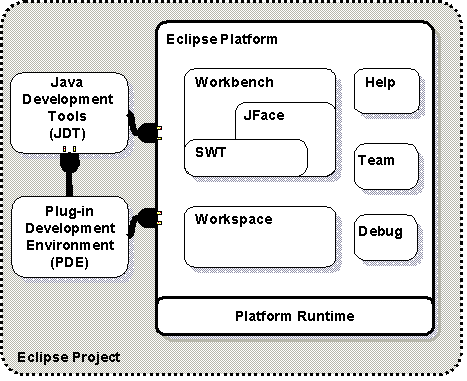
\includegraphics[width=1\textwidth]{images/EclipseArchitecture}
	\caption{Illustration of the modular architecture of Eclipse \cite{EclipseArchitecture}}
	\label{fig:EclipseArchitecture}
\end{figure}

A wide range of extensible and widely-used tools have been developed atop Eclipse including editors and launchers for many programming languages (Java, C, PHP, Ruby etc.), management tools for source code repositories such as CVS and SVN and modelling tools such as the Eclipse Modeling Framework (EMF) and the Graphical Modeling Framework (GMF). 

Due to its extensible nature, Eclipse enables users to implement supporting tools for new programming languages that integrate well with the rest of the platform with relatively little effort. Moreover, Eclipse is the platform of choice for MDE tools as the majority of contemporary MDE languages and frameworks provide Eclipse-based development tools. 

\subsection{Editors and Outline Views}
To enable users to compose programs in languages of the platform, language-specific editors aware of the concrete syntax of each language are required. Moreover, to enable users locate and correct syntactical errors, in-place markers that can highlight the lines that contain the error(s) are particularly useful. To maximize reuse, an abstract \emph{AbstractModuleEditor} class has been introduced (that extends the built-in \emph{TextEditor} Eclipse editor), which provides basic syntax highlighting services for keywords, comments, strings and numbers that apply to all Epsilon languages. Editors of individual languages (e.g. \emph{EclEditor} and \emph{EtlEditor}) extend this abstract editor to provide their specific keywords (e.g. \emph{compare} and \emph{transform} respectively). Similarly, a \emph{ModuleContentOutlinePage} has been introduced that implements a basic outline view providing services such as linking with editors and sorting (Figure \ref{fig:EditorAndOutline}, point 5). To specialize for a task-specific language, little customization (specifying icons and labels) is required. As an example, in Figure \ref{fig:EditorAndOutline}, the editor (1) and outline view (4), that provides a compact view of the transform-rules of an ETL module, are illustrated. Points (2) and (3) show how design-time errors are presented with the use of markers both in the editor and the \textit{problems} view of Eclipse.

\begin{landscape}
\begin{figure}
	\centering
		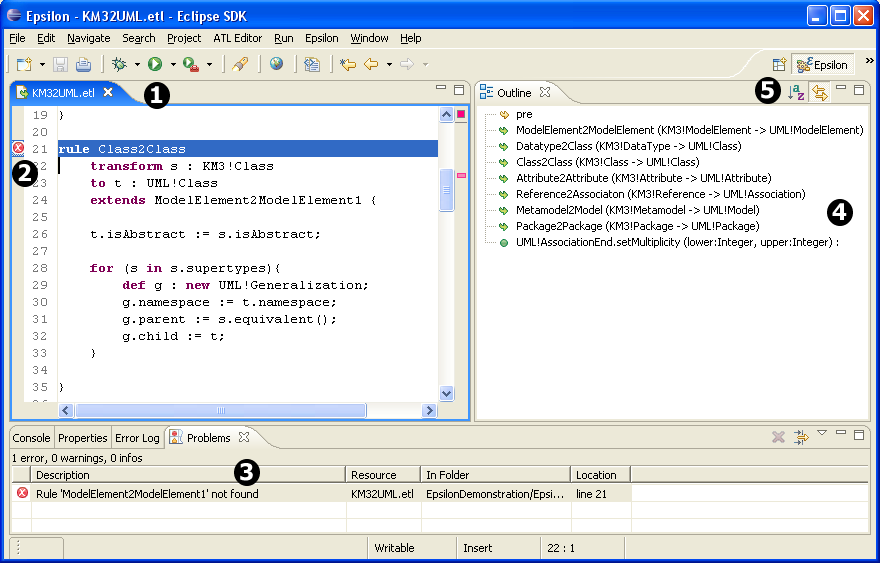
\includegraphics[width=20cm]{images/EditorAndOutline.png}
	\caption{ETL Editor and Outline View}
	\label{fig:EditorAndOutline}
\end{figure}
\end{landscape}

\subsection{Launch Configuration Interface}
Since languages in Epsilon are about managing models, a major sub-task when creating a launch configuration is to define the models it operates on. To achieve reuse and uniformity, separate tabs and dialogs have been implemented, each being able to configure models of a particular technology (e.g. EMF, MDR). These tabs are reused in the launch configuration interfaces of all Epsilon languages. Figure \ref{fig:LaunchConfiguration} illustrates the MDR and EMF model configuration tabs (1) and the dialog through which the name and extent (2), as well as the locations of the model and metamodel file (3), of an MDR model can be specified.

\begin{figure}
	\centering
		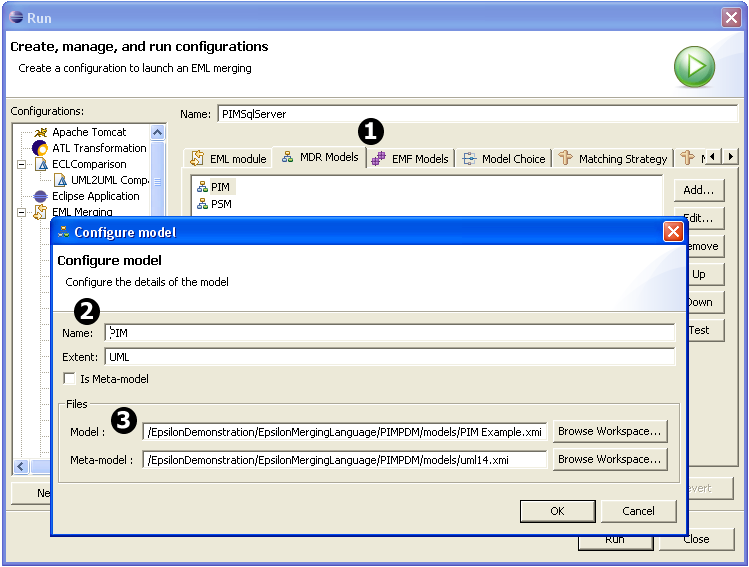
\includegraphics[width=1.0\textwidth]{images/LaunchConfiguration.png}
	\caption{EML Launch Configuration Interface}
	\label{fig:LaunchConfiguration}
\end{figure}

\subsection{The Epsilon Console}
To provide the user with feedback at run-time, a console dedicated to Epsilon languages has been implemented. Users can send textual messages to this console via the built-in \emph{print()} and \emph{println()} EOL operations. Moreover, as demonstrated in Figure \ref{fig:Console}, when a run-time error occurs during the execution of a module, an appropriate message (1) and a hyperlink (2) are displayed in the console to inform the user about the error. Clicking on the hyperlink navigates the user to the actual source of the error (3).

\begin{figure}
	\centering
		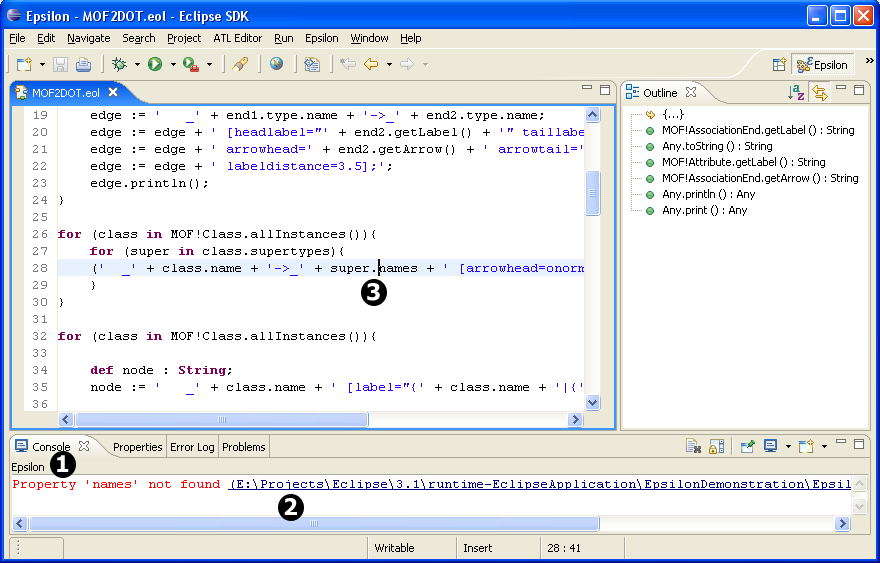
\includegraphics[width=1.0\textwidth]{images/Console.png}
	\caption{Epsilon Console}
	\label{fig:Console}
\end{figure}

\section{Workflow Implementation}
\label{sec:Implementation.Workflow}

As discussed in Chapter \ref{chp:Workflow}, the workflow mechanism for orchestrating individual Epsilon tasks into composite workflows has been designed atop the infrastructure provided by the ANT framework. Eclipse already provides out-of-the-box integration with ANT including extensible editors, views and launch configurations which have been extended to enable users to compose and execute workflows that involve instances of the Epsilon tasks presented in Sections \ref{sec:Workflow.Framework} and \ref{sec:Workflow.ModelManagementTasks}. Figure \ref{fig:ANTScreenshot1} demonstrates a content-assistance dialog that enables user to select one of the Epsilon tasks and figure \ref{fig:ANTScreenshot2} demonstrates the content assistance dialog that demonstrates the valid attributes for an ETL task.

\begin{figure}
	\centering
		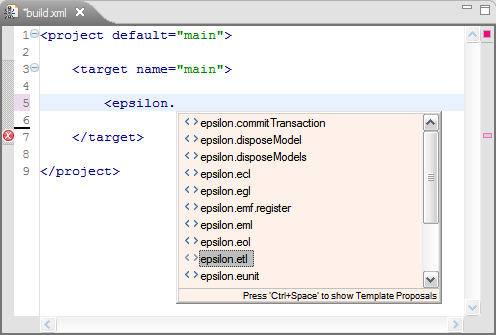
\includegraphics{images/ANTScreenshot1.png}
	\caption{Task content assistance dialog}
	\label{fig:ANTScreenshot1}
\end{figure}

\begin{figure}
	\centering
		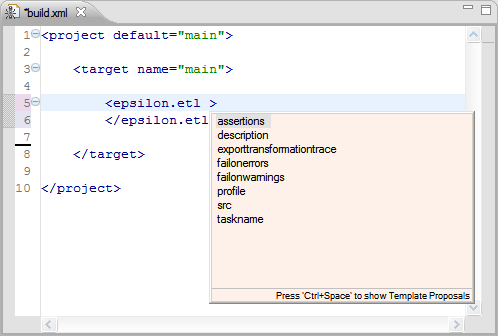
\includegraphics{images/ANTScreenshot2.png}
	\caption{Task attributes content assistance dialog}
	\label{fig:ANTScreenshot2}
\end{figure}

\section{Timeline and Availability}
\label{sec:Implementation.Timeline}

Initially, the source code and documentation of the implementation was maintained locally. Since May 2006 new binary versions of the execution engines and the Eclipse-based development tools have been released regularly through the author's departmental website. In November 2006, Epsilon was invited to become a component of the Eclipse GMT project. The Eclipse Generative Modeling Tools (GMT) project is the official research incubator project of the top-level Eclipse Modelling Project and hosts a small number of selected components (8 at the time of joining and 11 in May 2008). In January 2007 the source code was moved to the Eclipse CVS (concurrent version control) servers where it is since then accessible to the general public. Also, updated binary versions are regularly released as standalone archives and using the Eclipse Update Manager. Detailed instructions on how to obtain the source code and binaries are available in \cite{CVSInstallation} and \cite{BinariesInstallation} respectively.

\section{Chapter Summary}

This chapter has provided an overview of the reference implementation that enables users to compose and execute programs expressed using languages built atop Epsilon. Through this chapter, noteworthy implementation decisions such as the choice to implement a light-weight runtime and development tools atop the Eclipse platform have been discussed, and an outline of the timeline of the implementation process has been presented. This chapter concludes the design and implementation of Epsilon. The next chapter evaluates the validity of the hypothesis using a number of criteria, including a complex case study which has been realized using the reference implementation discussed here.